\documentclass[12pt]{repaso}
\grade{3$^\circ$ de Secundaria}
\cycle{2022-2023}
\subject{Matemáticas 3}
\guide{2}
\title{Repaso para el examen de la Unidad}
\aprendizajes{

    \begin{itemize}[leftmargin=*,label=\small\color{colorrds}\faIcon{user-graduate}]
        \item Resuelve problemas mediante la formulación y la solución
              algebraica de ecuaciones cuadráticas.
        \item Analiza y compara diversos tipos de variación a
              partir de sus representaciones tabular, gráfica y algebraica, que resultan de
              modelar situaciones y fenómenos de la Física y de otros contextos.
    \end{itemize}
}
\requisitos{
    \begin{itemize}
        \item Requisito 1
        \item Requisito 2
    \end{itemize}
}
\author{J. C. Melchor Pinto}

\begin{document}
\pagestyle{headandfoot}
%\thispagestyle{plain}
\addpoints
\INFO
%\printanswers
{\small
    \begin{multicols}{2}
        \include*{../blocks/block001}
    \end{multicols}
    \include*{../blocks/block002}
}
\begin{questions}
    \include*{../questions/question002}
    \newpage
    \include*{../questions/question004}
    %\newpage

    \question Lee con atención las siguientes situaciones y contesta lo que se te pide.

    \begin{parts}
        \begin{minipage}[t]{0.4\textwidth}
            \begin{figure}[H]
                \raggedright
                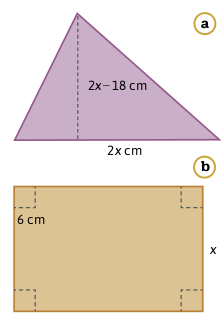
\includegraphics[width=0.9\linewidth]{../images/figuras2.7.png}
                \captionof{figure}{(a) Triángulo, (b) Pieza rectangular para armar una caja.}
                \label{fig:figuras2.7}
            \end{figure}
        \end{minipage}\hfill
        \begin{minipage}[t]{0.5\textwidth}
            \part[10] El triángulo de la figura \ref{fig:figuras2.7}a tiene área igual a 52 cm$^2$, encuentra las medidas de su base y de su altura.

            \begin{solutionbox}{3.5cm}

            \end{solutionbox}

            \part[10] Una pieza rectangular como la de la figura \ref{fig:figuras2.7}b es 4 cm más larga que ancha. Con ella se construye una caja de 840 cm$^3$ cortando un cuadrado
            en cada esquina y doblando los bordes. Escribe las medidas de la altura y el volumen de la caja, así como los lados de la pieza rectangular.
            \begin{solutionbox}{3.5cm}

            \end{solutionbox}
        \end{minipage}
        \setlength{\columnsep}{30pt} % I want the columnsep to be wider only on this page. Right now, nothing happens. The default 10pt is still being used.
        % \begin{multicols}{2}
        \part[10] El área de un rectángulo es 28 cm$^2$. Tiene 3 cm más de largo que de ancho. ¿Cuáles son sus dimensiones?

        \begin{solutionbox}{4cm}

        \end{solutionbox}

        \part[10] Un terreno rectangular tiene área de 750 m$^2$. Se coloca una cerca alrededor de los 110 m de perímetro. Calcula las dimensiones del terreno.

        \begin{solutionbox}{4cm}

        \end{solutionbox}

        % \part[5] Un rectángulo tiene el ancho más corto que el largo por 3 cm. El área de la figura es de 51 cm$^2$. ¿Qué medidas tiene?

        % \begin{solutionbox}{3cm}

        % \end{solutionbox}
    \end{parts}
\end{questions}
\end{document}